\huaxing{夯基达标}{保60\%}

\jx{1}{〔简单〕（知识点3）}{已知\(\left| \overrightarrow{a} \right| = 3\sqrt{2},\left| \overrightarrow{b} \right| = 4,\overrightarrow{m} = \overrightarrow{a} + \overrightarrow{b},\overrightarrow{n} = \overrightarrow{a} + \lambda\overrightarrow{b},\left\langle \overrightarrow{a},\overrightarrow{b} \right\rangle = 135{^\circ},\overrightarrow{m}\bot\overrightarrow{n}\) ，则λ＝\kongbai{}．}

\jx{2}{〔简单〕（知识点2）}{化简\(\overrightarrow{AB} + \overrightarrow{BC} - \overrightarrow{AD}\)＝（\quad）}

\bindopt A．\(\overrightarrow{DB}\)；B．\(\overrightarrow{BD}\)；C．\(\overrightarrow{DC}\)；D．\(\overrightarrow{CD}\)

\jx{3}{〔简单〕（知识点2）}{在平行六面体\(ABCD - A_{1}B_{1}C_{1}D_{1}\)中，已知\(\overrightarrow{AB} = \overrightarrow{a}\)，\(\overrightarrow{AD} = \overrightarrow{b}\)，\(\overrightarrow{AA_{1}} = \overrightarrow{c}\)，则\(\overrightarrow{A_{1}D} =\)\kongbai{}，\(\overrightarrow{AC_{1}} =\)\kongbai{}．（用\(\overrightarrow{a}\)，\(\overrightarrow{b}\)，\(\overrightarrow{c}\)表示）}

\jx{4}{〔简单〕（知识点1）}{有下列说法：①零向量与任意向量共线；②模相等且方向相反的两个向量互为相反向量；③共线向量所在的直线必重合；④相等向量的起点必相同．其中正确的是（\quad）}

\bindopt A．①②；B．①②③；C．②③；D．①③④

\jx{5}{〔简单〕（知识点3）}{已知\(\overrightarrow{a}\)，\(\overrightarrow{b}\)为非零向量，则\(\overrightarrow{a} \cdot \overrightarrow{b} < 0\)是\(\langle \overrightarrow{a},\overrightarrow{b} \rangle\)为钝角的（\quad）}

\optgrid{A．充分而不必要条件； & B．必要而不充分条件； \\
C．充要条件； & D．既不充分也不必要条件}

\huaxing{提能进阶}{保80\%}

\jxfig{6}{〔中档〕（知识点3）}{如图，在正方体\(ABCD - A_{1}B_{1}C_{1}D_{1}\)中，求向量\(\overrightarrow{A_{1}B}\)与\(\overrightarrow{BC_{1}}\)夹角的大小．}{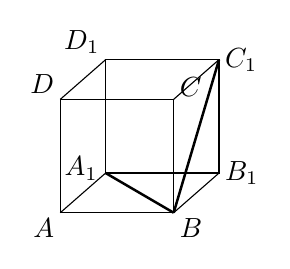
\begin{tikzpicture}[baseline=(current bounding box.north),line width=0.4pt,x=1mm,y=1mm,scale=0.72]
\coordinate (A) at (0,0);\coordinate (B) at (20,0);\coordinate (C) at (20,20);\coordinate (D) at (0,20);
\coordinate (A1) at (8,7);\coordinate (B1) at (28,7);\coordinate (C1) at (28,27);\coordinate (D1) at (8,27);
\draw (A)--(B)--(C)--(D)--cycle;
\draw (A1)--(B1)--(C1)--(D1)--cycle;
\draw (A)--(A1);\draw (B)--(B1);\draw (C)--(C1);\draw (D)--(D1);
\draw[line width=0.9pt] (A1)--(B);\draw[line width=0.9pt] (B)--(C1);
\node[anchor=north east,inner sep=1pt] at (-0.5,-0.5) {\figfont $A$};
\node[anchor=north west,inner sep=1pt] at (20.5,-0.5) {\figfont $B$};
\node[anchor=south west,inner sep=1pt] at (20.5,20) {\figfont $C$};
\node[anchor=south east,inner sep=1pt] at (-0.5,20.5) {\figfont $D$};
\node[anchor=east,inner sep=1pt] at (7.2,7.8) {\figfont $A_1$};
\node[anchor=west,inner sep=1pt] at (28.5,7) {\figfont $B_1$};
\node[anchor=west,inner sep=1pt] at (28.5,27) {\figfont $C_1$};
\node[anchor=south east,inner sep=1pt] at (7.5,27.5) {\figfont $D_1$};
\end{tikzpicture}}

\liubai{3}

\jx{7}{〔中档〕（知识点3）}{已知空间向量\(\overrightarrow{a}\)，\(\overrightarrow{b}\)满足\(\left| \overrightarrow{a} \right| = 3\)，\(\left| \overrightarrow{b} \right| = 2\)，\(\langle \overrightarrow{a},\overrightarrow{b} \rangle = 120^{\circ}\)，则\(\left| \overrightarrow{a} \right|\cos\langle \overrightarrow{a},\overrightarrow{b} \rangle =\)\kongbai{}，\(\overrightarrow{a}\)在\(\overrightarrow{b}\)上的投影向量为\kongbai{}．}

\jx{8}{〔中档〕（知识点3）}{已知\(\overrightarrow{a}\)，\(\overrightarrow{b}\)，\(\overrightarrow{c}\)为空间向量，则下列各式一定成立的是（\quad）}

\bindopt A．若\(\overrightarrow{a} \cdot \overrightarrow{b} = 0\)，则\(\overrightarrow{a} \perp \overrightarrow{b}\)；

\bindopt B．\(\left( \overrightarrow{a} \cdot \overrightarrow{b} \right) \cdot \overrightarrow{c} = \overrightarrow{a} \cdot \allowbreak\left( \overrightarrow{b} \cdot \overrightarrow{c} \right)\)；

\bindopt C．\(\left| \overrightarrow{a} \cdot \overrightarrow{b} \right| \leq \left| \overrightarrow{a} \right| \cdot \allowbreak\left| \overrightarrow{b} \right|\)；

\bindopt D．若\(\overrightarrow{a} \cdot \overrightarrow{b} > 0\)，则\(\langle \overrightarrow{a},\overrightarrow{b} \rangle\)必为锐角

\jx{9}{〔中档〕★（知识点3）}{已知空间向量\(\overrightarrow{a}\)，\(\overrightarrow{b}\)满足\(\left| \overrightarrow{a} \right| = 2\)，\(\left| \overrightarrow{b} \right| = 3\)，则\(\left| \overrightarrow{a} + \overrightarrow{b} \right|^{2} + \left| \overrightarrow{a} - \overrightarrow{b} \right|^{2} =\)（\quad）}

\bindopt A．26；B．13；C．25；D．20

\huaxing{冲刺突破}{冲100\%}

\jx{10}{〔中档〕（知识点2）}{在空间四边形\(ABCD\)中，\(E\)，\(H\)分别是棱\(AB\)，\(AD\)的中点，\(F\)，\(G\)分别是棱\(CB\)，\(CD\)上的点，且\(\overrightarrow{CF} = \frac{1}{3}\overrightarrow{CB}\)，\(\overrightarrow{CG} = \frac{1}{3}\overrightarrow{CD}\)．求证：四边形\(EFGH\)是梯形．}

\liubai{3}

\jx{11}{〔中档〕★（知识点3）}{如图，在平行六面体\(ABCD - A_{1}B_{1}C_{1}D_{1}\)中，各棱长均为2，且从同一顶点\(A\)出发的三条棱两两夹角均为\(60^{\circ}\)．（1）求对角线\(AC_{1}\)与\(BD_{1}\)的长；（2）求\(\overrightarrow{AC_{1}} \cdot \overrightarrow{BD_{1}}\)的值．}

\figblock{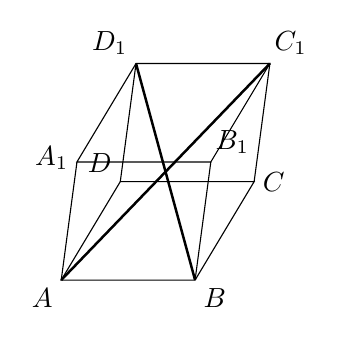
\begin{tikzpicture}[line width=0.4pt,x=1mm,y=1mm]
\coordinate (A) at (0,0);\coordinate (B) at (17,0);\coordinate (D) at (7.5,12.5);\coordinate (A1) at (2,15);
\coordinate (C) at (24.5,12.5);\coordinate (B1) at (19,15);\coordinate (C1) at (26.5,27.5);\coordinate (D1) at (9.5,27.5);
\draw (A)--(B)--(C)--(D)--cycle;
\draw (A1)--(B1)--(C1)--(D1)--cycle;
\draw (A)--(A1);\draw (B)--(B1);\draw (C)--(C1);\draw (D)--(D1);
\draw[line width=0.9pt] (A)--(C1);\draw[line width=0.9pt] (B)--(D1);
\node[anchor=north east,inner sep=1.5pt] at (-0.5,-0.5) {\figfont $A$};
\node[anchor=north west,inner sep=1.5pt] at (17.5,-0.5) {\figfont $B$};
\node[anchor=west,inner sep=1.5pt] at (25,12.5) {\figfont $C$};
\node[anchor=south east,inner sep=1.5pt] at (7,13) {\figfont $D$};
\node[anchor=east,inner sep=1.5pt] at (1.5,15.5) {\figfont $A_1$};
\node[anchor=south west,inner sep=1.5pt] at (19,15.5) {\figfont $B_1$};
\node[anchor=south west,inner sep=1.5pt] at (26.5,28) {\figfont $C_1$};
\node[anchor=south east,inner sep=1.5pt] at (9,28) {\figfont $D_1$};
\end{tikzpicture}}
